\documentclass[journal,12pt,twocolumn]{IEEEtran}

\usepackage{setspace}
\usepackage{gensymb}
\singlespacing
\usepackage[cmex10]{amsmath}
\usepackage[table]{xcolor}
\usepackage{amsthm}

\usepackage{mathrsfs}
\usepackage{txfonts}
\usepackage{stfloats}
\usepackage{bm}
\usepackage{cite}
\usepackage{cases}
\usepackage{subfig}

\usepackage{longtable}
\usepackage{multirow}

\usepackage{enumitem}
\usepackage{mathtools}
\usepackage{steinmetz}
\usepackage{tikz}
\usepackage{circuitikz}
\usepackage{verbatim}
\usepackage{tfrupee}
\usepackage[breaklinks=true]{hyperref}
\usepackage{graphicx}
\usepackage{tkz-euclide}


\usetikzlibrary{calc,math}
\usepackage{listings}
    \usepackage{color}                                            %%
    \usepackage{array}                                            %%
    \usepackage{longtable}                                        %%
    \usepackage{calc}                                             %%
    \usepackage{multirow}                                         %%
    \usepackage{hhline}                                           %%
    \usepackage{ifthen}                                           %%
    \usepackage{lscape}     
\usepackage{multicol}
\usepackage{chngcntr}

\DeclareMathOperator*{\Res}{Res}

\renewcommand\thesection{\arabic{section}}
\renewcommand\thesubsection{\thesection.\arabic{subsection}}
\renewcommand\thesubsubsection{\thesubsection.\arabic{subsubsection}}

\renewcommand\thesectiondis{\arabic{section}}
\renewcommand\thesubsectiondis{\thesectiondis.\arabic{subsection}}
\renewcommand\thesubsubsectiondis{\thesubsectiondis.\arabic{subsubsection}}


\hyphenation{op-tical net-works semi-conduc-tor}
\def\inputGnumericTable{}                                 %%

\lstset{
%language=C,
frame=single, 
breaklines=true,
columns=fullflexible
}
\begin{document}

\newcommand{\BEQA}{\begin{eqnarray}}
\newcommand{\EEQA}{\end{eqnarray}}
\newcommand{\define}{\stackrel{\triangle}{=}}
\bibliographystyle{IEEEtran}
\raggedbottom
\setlength{\parindent}{0pt}
\providecommand{\mbf}{\mathbf}
\providecommand{\pr}[1]{\ensuremath{\Pr\left(#1\right)}}
\providecommand{\qfunc}[1]{\ensuremath{Q\left(#1\right)}}
\providecommand{\sbrak}[1]{\ensuremath{{}\left[#1\right]}}
\providecommand{\lsbrak}[1]{\ensuremath{{}\left[#1\right.}}
\providecommand{\rsbrak}[1]{\ensuremath{{}\left.#1\right]}}
\providecommand{\brak}[1]{\ensuremath{\left(#1\right)}}
\providecommand{\lbrak}[1]{\ensuremath{\left(#1\right.}}
\providecommand{\rbrak}[1]{\ensuremath{\left.#1\right)}}
\providecommand{\cbrak}[1]{\ensuremath{\left\{#1\right\}}}
\providecommand{\lcbrak}[1]{\ensuremath{\left\{#1\right.}}
\providecommand{\rcbrak}[1]{\ensuremath{\left.#1\right\}}}
\theoremstyle{remark}
\newtheorem{rem}{Remark}
\newcommand{\sgn}{\mathop{\mathrm{sgn}}}
\providecommand{\abs}[1]{\vert#1\vert}
\providecommand{\res}[1]{\Res\displaylimits_{#1}} 
\providecommand{\norm}[1]{\lVert#1\rVert}
%\providecommand{\norm}[1]{\lVert#1\rVert}
\providecommand{\mtx}[1]{\mathbf{#1}}
\providecommand{\mean}[1]{E[ #1 ]}
\providecommand{\fourier}{\overset{\mathcal{F}}{ \rightleftharpoons}}
%\providecommand{\hilbert}{\overset{\mathcal{H}}{ \rightleftharpoons}}
\providecommand{\system}{\overset{\mathcal{H}}{ \longleftrightarrow}}
	%\newcommand{\solution}[2]{\textbf{Solution:}{#1}}
\newcommand{\solution}{\noindent \textbf{Solution: }}
\newcommand{\cosec}{\,\text{cosec}\,}
\providecommand{\dec}[2]{\ensuremath{\overset{#1}{\underset{#2}{\gtrless}}}}
\newcommand{\myvec}[1]{\ensuremath{\begin{pmatrix}#1\end{pmatrix}}}
\newcommand{\mydet}[1]{\ensuremath{\begin{vmatrix}#1\end{vmatrix}}}
\numberwithin{equation}{subsection}
\makeatletter
\@addtoreset{figure}{problem}
\makeatother
\let\StandardTheFigure\thefigure
\let\vec\mathbf
\renewcommand{\thefigure}{\theproblem}
\def\putbox#1#2#3{\makebox[0in][l]{\makebox[#1][l]{}\raisebox{\baselineskip}[0in][0in]{\raisebox{#2}[0in][0in]{#3}}}}
     \def\rightbox#1{\makebox[0in][r]{#1}}
     \def\centbox#1{\makebox[0in]{#1}}
     \def\topbox#1{\raisebox{-\baselineskip}[0in][0in]{#1}}
     \def\midbox#1{\raisebox{-0.5\baselineskip}[0in][0in]{#1}}
\vspace{3cm}
\title{Assignment-1}%number
\author{Lanka Prasanna - CS20BTECH11029}
\maketitle
\newpage
\bigskip
\item{\textbf{Problem:}}
\\
Consider the experiment of tossing a coin. If the coin shows head, toss it again but if it shows tail, then throw a die. Find the conditional probability of the event that ``the die shows a number greater than 4" given that ``there is at least one tail".
\item{\textbf{Solution:}}
\\
Given that a coin is tossed.
\\If coin shows head, it is tossed again.
\\If it shows tail, then a die is thrown.
\\
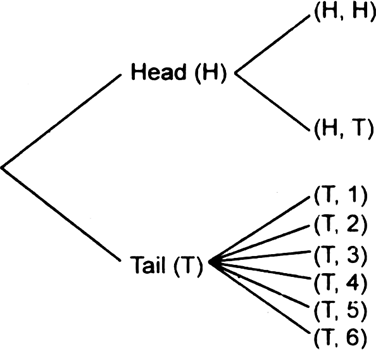
\includegraphics[scale=0.75]{MAEN12065250}
\\\text{Different probabilities are given by}
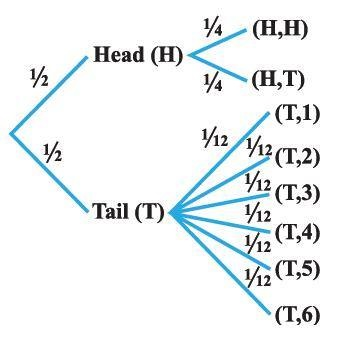
\includegraphics[scale=0.75]{fig1.jpg}


\setlength{\arrayrulewidth}{1mm}
\setlength{\tabcolsep}{10pt}
\renewcommand{\arraystretch}{2}
{\rowcolors{3}{green!80!yellow!50}{green!70!yellow!40}
\begin{tabular}{ |p{3cm}|p{3cm}|  }
\hline
\multicolumn{2}{|c|}{Probabilities } \\
\hline
Event &  Probability\\
\hline
(H,H) & $\frac{1}{2}.\frac{1}{2}=\frac{1}{4}$\\
(H,T) & $\frac{1}{2}.\frac{1}{2}=\frac{1}{4}$\\
(T,1) & $\frac{1}{2}.\frac{1}{6}=\frac{1}{12}$\\
(T,2) & $\frac{1}{2}.\frac{1}{6}=\frac{1}{12}$\\
(T,3) & $\frac{1}{2}.\frac{1}{6}=\frac{1}{12}$\\
(T,4) & $\frac{1}{2}.\frac{1}{6}=\frac{1}{12}$\\
(T,5) & $\frac{1}{2}.\frac{1}{6}=\frac{1}{12}$\\
(T,6) & $\frac{1}{2}.\frac{1}{6}=\frac{1}{12}$\\
\hline
\end{tabular}
}
\\\\

Let X $\in$ $\{0,1\}$ be the random variable such that 1 represents occurrence of tail,0 represents occurrence of head when coin is tossed.
\begin{table}[ht]
\caption{Probability distribution for values of X}
\begin{center}
    \begin{tabular}{|c|c|}
    \hline
    X & P(X)\\
    \hline
    1 & $\frac{1}{2}$ \\
    \hline
    0 & $\frac{1}{2}$\\
    \hline
    \end{tabular}
\end{center} 
\end{table}
\\Let Y denotes the getting a number on the die thrown, then the probability distribution is
\begin{table}[ht]
\caption{Probability distribution for values of Y}
\begin{center}
    \begin{tabular}{|c|c|c|c|c|c|c|}
    \hline
    Y & 1 & 2 & 3 & 4 & 5 & 6 \\
    \hline
    P(Y) & $\frac{1}{6}$ & $\frac{1}{6}$ & $\frac{1}{6}$ & $\frac{1}{6}$ & $\frac{1}{6}$ & $\frac{1}{6}$  \\
    \hline
    \end{tabular}
\end{center} 
\end{table}
\\\\\\\\\\\\
Pr$(X=1)$\\
= Pr$(H,T)$+Pr$(T,1)$+Pr$(T,2)$+Pr$(T,3)$+Pr$(T,4)$+Pr$(T,5)$+Pr$(T,6)$ \\ 
=$\frac{1}{4}$+$\frac{1}{12}$+$\frac{1}{12}$+$\frac{1}{12}$+$\frac{1}{12}$+$\frac{1}{12}$+$\frac{1}{12}$\\
=$\frac{1}{4}$+$\frac{6}{12}$\\
=$\frac{3}{4}$\\\\
Pr$(X=1,Y>4)$\\
=Pr$(T,5)$+Pr$(T,6)$\\
=$\frac{1}{12}$+$\frac{1}{12}$\\
=$\frac{1}{6}$\\\\
We need Pr$(Y>4|X=1)$\\
We know that
\begin{equation}
   \text{Pr}(Y>4|X=1)= \frac{\text{Pr}(Y>4,X=1)}{\text{Pr}(X=1)} 
\end{equation}
\begin{equation}
  \text{Pr}(Y>4|X=1)= \frac{\frac{1}{6}}{\frac{3}{4}}=\frac{2}{9}
\end{equation}
\therefore \text{The required probability is } \fbox{$\frac{2}{9}$}\\\\
\text{Download all latex codes from:} 
\begin{lstlisting}

\end{lstlisting}
\end{document}
